% !TeX root = Thesis.tex

\begin{figure}[!htbp]
\centering

\begin{tikzpicture}[level distance=1.25cm,
  level 1/.style={sibling distance=8cm},
  level 2/.style={sibling distance=4cm},
  level 3/.style={sibling distance=3cm}]
  \node {n=5}
    child { node {$H$ exists}
      child { node {$\underset{\raisebox{-0.8em}{11}}{\text{LP integer}}$} }
      child { node {$\underset{\raisebox{-0.8em}{0}}{\text{LP fractional}}$} 
        child { node {$\underset{\raisebox{-0.8em}{0}}{\text{Rounding}}$}  }
        child { node {$\underset{\raisebox{-0.8em}{0}}{\text{Infeasible}}$}  }
      }
    }
    child { node {$H$ does not exist}
      child { node {$\underset{\raisebox{-0.8em}{20}}{\text{LP infeasible}}$} }
      child { node {$\underset{\raisebox{-0.8em}{3}}{\text{LP fractional}}$} 
        child { node {$\underset{\raisebox{-0.8em}{0}}{\text{Rounding}}$}  }
        child { node {$\underset{\raisebox{-0.8em}{3}}{\text{Infeasible}}$}  }
      }
    };
\end{tikzpicture}

\begin{tikzpicture}[level distance=1.25cm,
  level 1/.style={sibling distance=8cm},
  level 2/.style={sibling distance=4cm},
  level 3/.style={sibling distance=3cm}]
  \node {n=6}
    child { node {$H$ exists}
      child { node {$\underset{\raisebox{-0.8em}{22}}{\text{LP integer}}$} }
      child { node {$\underset{\raisebox{-0.8em}{6}}{\text{LP fractional}}$} 
        child { node {$\underset{\raisebox{-0.8em}{6}}{\text{Rounding}}$}  }
        child { node {$\underset{\raisebox{-0.8em}{0}}{\text{Infeasible}}$}  }
      }
    }
    child { node {$H$ does not exist}
      child { node {$\underset{\raisebox{-0.8em}{107}}{\text{LP infeasible}}$} }
      child { node {$\underset{\raisebox{-0.8em}{21}}{\text{LP fractional}}$} 
        child { node {$\underset{\raisebox{-0.8em}{0}}{\text{Rounding}}$}  }
        child { node {$\underset{\raisebox{-0.8em}{21}}{\text{Infeasible}}$}  }
      }
    };
\end{tikzpicture}

\begin{tikzpicture}[level distance=1.25cm,
  level 1/.style={sibling distance=8cm},
  level 2/.style={sibling distance=4cm},
  level 3/.style={sibling distance=3cm}]
  \node {n=7}
    child { node {$H$ exists}
      child { node {$\underset{\raisebox{-0.8em}{43}}{\text{LP integer}}$} }
      child { node {$\underset{\raisebox{-0.8em}{34}}{\text{LP fractional}}$} 
        child { node {$\underset{\raisebox{-0.8em}{30}}{\text{Rounding}}$}  }
        child { node {$\underset{\raisebox{-0.8em}{4}}{\text{Infeasible}}$}  }
      }
    }
    child { node {$H$ does not exist}
      child { node {$\underset{\raisebox{-0.8em}{767}}{\text{LP infeasible}}$} }
      child { node {$\underset{\raisebox{-0.8em}{200}}{\text{LP fractional}}$} 
        child { node {$\underset{\raisebox{-0.8em}{0}}{\text{Rounding}}$}  }
        child { node {$\underset{\raisebox{-0.8em}{200}}{\text{Infeasible}}$}  }
      }
    };
\end{tikzpicture}

\begin{tikzpicture}[level distance=1.25cm,
  level 1/.style={sibling distance=8cm},
  level 2/.style={sibling distance=4cm},
  level 3/.style={sibling distance=3cm}]
  \node {n=8}
    child { node {$H$ exists}
      child { node {$\underset{\raisebox{-0.8em}{102}}{\text{LP integer}}$} }
      child { node {$\underset{\raisebox{-0.8em}{205}}{\text{LP fractional}}$} 
        child { node {$\underset{\raisebox{-0.8em}{144}}{\text{Rounding}}$}  }
        child { node {$\underset{\raisebox{-0.8em}{61}}{\text{Infeasible}}$}  }
      }
    }
    child { node {$H$ does not exist}
      child { node {$\underset{\raisebox{-0.8em}{9380}}{\text{LP infeasible}}$} }
      child { node {$\underset{\raisebox{-0.8em}{2659}}{\text{LP fractional}}$} 
        child { node {$\underset{\raisebox{-0.8em}{0}}{\text{Rounding}}$}  }
        child { node {$\underset{\raisebox{-0.8em}{2659}}{\text{Infeasible}}$}  }
      }
    };
\end{tikzpicture}

\caption{LP outcomes for different values of $n$ on the linear program with max objective function 
and using rounding for fractional solutions.}
\label{fig::rounding_max_objective_function_diagram}
\end{figure}